                                                                                                              \begin{enumerate}
\item In \figref{fig:quadrilateralABCD}, a quadrilateral $ABCD$ is drawn to circumscribe a circle with center $O$, such that the sides $AB, BC, CD,$ and $DA$ touch the circle at points $P, Q, R$ and $S$ respectively. Prove that $AB + CD = BC + DA$.
    \begin{figure}[H]
        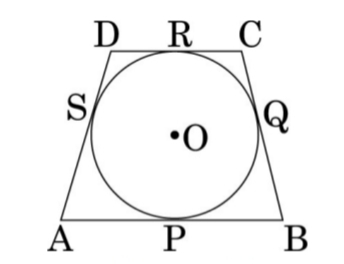
\includegraphics[width=\columnwidth]{figs/quadrilateralABCD.jpg}
        \caption{Quadrilateral ABCD}
        \label{fig:quadrilateralABCD}
    \end{figure}
\item In \figref{fig:coneontopofcylinder}, a tent is in the shape of a cylinder surmounted by a conical top of the same diameter. If the height and diameter of the cylindrical part are $2.1 m$ and $3 m$ respectively, and the slant height of the conical part is $2.8 m$, find the cost of the canvas needed to make the tent if the canvas is available at the rate of $\rupee 500/ m^2$. (Use $\pi = \frac{22}{7}$)
    \begin{figure}[H]
        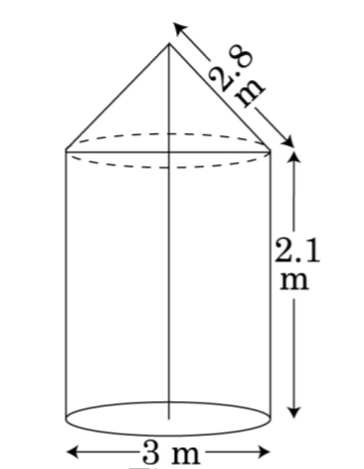
\includegraphics[width=\columnwidth]{figs/coneontopofcylinder.jpg}
        \caption{Cone on top of a cylinder}
        \label{fig:coneontopofcylinder}
    \end{figure}

    \item A sphere of diameter $12 cm$ is dropped in a right circular cylindrical vessel, partly filled with water. If the sphere is completely submerged in water, the water level in the cylindrical vessel rises by $3\frac{5}{9} cm$. Find the diameter of the cylindrical vessel.

    \item Due to heavy floods in a state, thousands were rendere
d homeless. Fifty schools collectively offered to provide place and canvas for $1500$ tents to be fixed by the government and decided to share the whole expenditure equally. The lower part of each tent is cylindrical with a base radius of $2.8 m$ and height $3.5 m$, with a conical upper part of the same base radius but of height $2.1 m$. If the canvas used to make the tents costs $\rupee 120/ m^2$, find the amount shared by each school to set up the tents. What value is generated by the above problem? (Use $\pi = \frac{22}{7} $)                                          
    \item In \figref{fig:triangleABC}, the vertices of $\triangle ABC$ are $A(4, 6), B(1, 5)$ and $C(7, 2)$. A line segment $DE$ is drawn to intersect the sides $AB$ and $AC$ at $D$ and $E$ re
spectively such that $\frac{AD}{AB} = \frac{AE}{AC} = \frac{1}{3}$. Calculate the area of $\triangle ADE$ and compare it with the area of $\triangle ABC$.                                          \begin{figure}[H]                                                   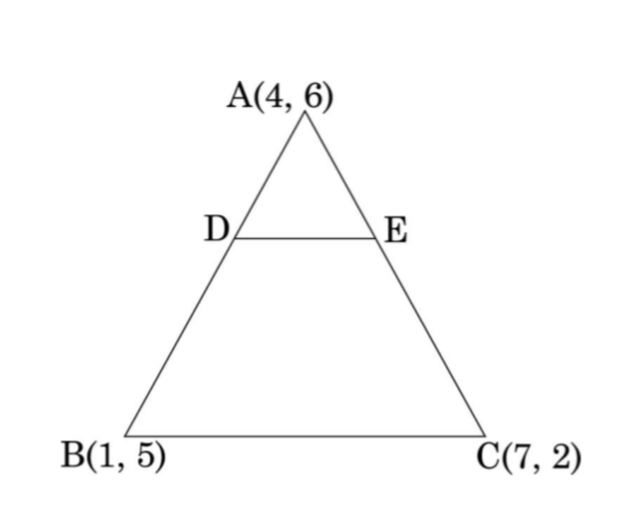
\includegraphics[width=\columnwidth]{figs/triangleABC.jpg}         \caption{Triangle ABC}                                          \label{fig:triangleABC}                                     \end{figure}

\item Draw a triangle with sides $5 cm, 6 cm$ and $7 cm$. T
    hen draw another triangle whose sides are $\frac{4}{5}$ of the
    corresponding sides of the first triangle.
								\end{enumerate}                                                 
